\section{A new corpus for natural language inference}\label{sec:discussion}

need for new corpus

Our ultimate aim in this work is to develop supervised models for sentence representation that can accurately capture natural language meaning. While sentiment tasks like SST have provided a useful testbed for sentence representation models, sentiment labeling only requires that models be able to encode a small piece of the full expressive capacity of language. We claim that the task of natural language inference (also called recognizing textual entailment, or RTE) is significantly more demanding, and that strong performance on this task is good evidence of a model's overall strength in sentence representation.


\subsection{Grounding with imagined images}

Quote from SICK paper \cite{marelli2014sick}:

\begin{quote}
Not unreasonably, subjects found that, say, \ii{A woman is wearing an Egyptian headdress} does not contradict \ii{A woman is wearing an Indian headdress}, since one could easily imagine both sentences truthfully uttered to refer to a single scene where two different women are wearing different headdresses. In the future, a higher proportion of CONTRADICTION labels could be elicited by using grammatical and possibly visual cues (pictures) encouraging co-indexing of the entities in the two sentences.
\end{quote}

\subsection{Data collection}

\subsection{Data validation}

\subsection{Statistics}

what's new
- size
- grounding

data will be freely available

SICK presented an important challenge, we try to deliver on it.

aim to surpass sick in both size and r consistency

Since our goal is to evaluate the quality of the single sentence representations in our model, we train an entailment classifier that has access only to the output of our sentence representation model, and not to any of the word or phrase representations that it used. We encourage future users of this corpus to evaluate their models in this way when possible. Our classifier is simply a stack of three 100d (NONLIN) layers, with the bottom layer taking the concatenated sentence representations as input and the top layer feeding a softmax classifier, all trained jointly with the representation model itself.

We use captions from the Flickr30k corpus \cite{hodoshimage} as the left hand side of each relation pair. That corpus ...

We randomly selected individual captions from that corpus to use in our own corpus, though in the interest of encouraging more complex source sentences without discarding too much source data, we downsample sentences with lengths of under 90 characters so that these sentences make up only half of our corpus, rather than the original 69\%.

... licencing ...

The instructions for this phase were integrated into the design of the data collection interface. The text of those instructions is shown in Figure~\ref{instructions-1}. We chose to use three classes, corresponding to ENTAILMENT, CONTRADICTION, and NEUTRAL classes used in SICK.

\begin{figure}
\footnotesize
% \toprule
The Stanford University NLP Group is collecting data for use in research on computer understanding of English. We appreciate your help!

We will show you the caption for a photo. We will not show you the photo. Using only the caption and what you know about the world:
\begin{itemize}
\item Write one alternate caption that is \textbf{definitely} a \textbf{true} description of the photo. \ii{Example: For the caption "Two dogs are running through a field." you could write "There are animals outdoors."}
\item Write one alternate caption that \textbf{might be} a \textbf{true} description of the photo. \ii{Example: For the caption "Two dogs are running through a field." you could write "There are animals outdoors."}
\item Write one alternate caption that is \textbf{definitely} a \textbf{false} description of the photo. \ii{Example: For the caption "Two dogs are running through a field." you could write "There are animals outdoors." This is different from the maybe correct category because its impossible for the dogs to be both running and sitting.}
\end{itemize}
\textbf{Problems} (optional)   If something is wrong with the caption that makes it difficult to understand, do your best above and let us know here.
% \bottomrule
\caption{\label{instructions-1}Examples of training data from the newly collected entailment corpus.}
\end{figure}


We posted 15.5k ImageFlickr captions. We showed each of the first 10k captions to five workers, yielding fifteen reponse sentences per source caption, with five assigned to each of the three labels. Then, to ensure maximal diversity in the test set, we showed the remaining 5.5k source captions to one worker each,  yielding only three responses per source caption.

We collected 143,023 pairs, after excluding less than 100 worker responses in which the worker reported that they could not understand the source caption, or in which a field was accidentally left blank. The average worker response sentence was 7.8 words long. 1100 workers participated in the task.

pre-verification distribution:

Recompute after removing blanks:
29305 contra
29304 neut
29305 ent

% ditto examples
%
\begin{table*}
  \centering\footnotesize
  \begin{tabular}{p{6.5cm}cp{6.5cm}}
  \toprule
A busy street with building lined up and people walking down the street outside and nighttime. &\ii{entailment}	&People lined up\\
\rule{0pt}{3ex}Two men stand in an electric outdoor lift. &\ii{neutral}	& The two men are inspectors for the FDA, waiting to inspect the second level of the pharmaceutical plant.\\
\rule{0pt}{3ex}A young redheaded girl, wearing a yellow shirt, black pants, and sneakers, jumping in a grassy field with blue skies and wispy clouds in the background. &\ii{entailment}	& A girl jumps in a grassy field\\
\rule{0pt}{3ex}A crowd of people, one with a guitar, are standing in the street under the 7th Avenue street sign. &\ii{neutral}	& The crowd listening to the man play guitar.\\
\rule{0pt}{3ex}A woman wearing bike shorts and a skirt is riding a bike and carrying a shoulder bag.  &\ii{contradiction}& A woman driving a car.\\
    \bottomrule
  \end{tabular}
  \caption{\label{examplesofscedata}The instructions presented to workers during data collection.}
\end{table*}


% Screenshot from phase 1


% Screenshot from phase 2

The data is freely available at (POST DATA), and is released under a CreativeCommons
Attribution-ShareAlike licence, which is the same licence used for the Flickr30k source captions.

\paragraph{Validation}

The majority of the sentence pairs in the corpus have not been reviewed by anyone since their construction as part of the data collection Mechanical Turk task, except to remove blank responses and responses some pairs which the original author flagged for review. However, in order to measure the quality of our corpus, and in order to construct maximally useful testing and development sets, we did perform an additional round of validation for about 54k examples.

This validation phase is not fundamentally different from the Mechanical Turk labeling task used for the SICK entailment data: we present workers with pairs of sentences (in our case, in batches of five at a time), and ask them to choose a single label for each pair. We supplied each pair to four annonators, yielding five labels per pair including the label used by the original composer of the pair. 

The results of this validation process are summarized in Fig.~\ref{validation-stats}. For each pair that we validated, we chose a gold label. If any one of the three labels was chosen by at least three of the five annotators, that label is the gold label. If there was no such consensus, which occurred in about 0.2\% of cases, we chose the label `-'. While these unlabeled examples are included in the corpus distribution, they are unlikely to be helpful for the core classification task of NLI, and we 

TODO: Data filtering? Data re-labeling?

\begin{figure}
\footnotesize
%\toprule
TODO: VALIDATION INSTRUCTIONS
%\bottomrule\\

\caption{\label{instructions-2}The instructions presented to workers during data validation.}
\end{figure}

\begin{figure}
\center
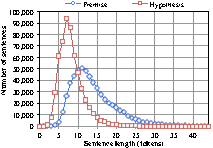
\includegraphics[width=3.05in]{length_dist}
    % From 1.0rc2
\caption{\label{b-table}The distribution of sentence length.} 
\end{figure}

\begin{table}
\center
  %\setlength{\tabcolsep}{15pt}
  %\renewcommand{\arraystretch}{1.2}
  \begin{tabular}{l l} 
    \toprule
Pairs in corpus & 570,157\\
Training pairs &  550,159\\
Dev pairs &  9,999\\
Test pairs &  9,999\\
\midrule
Premise mean token count & 14.1\\
Hypothesis mean token count & 8.3 \\
\midrule
Premise complete sentences & 70.2 ??\%\\
Hypothesis complete sentences & 75.4 ??\%\\
    \bottomrule
  \end{tabular}
    % From 1.0rc2
\caption{\label{validation-stats}Key statistics for the raw sentence pairs. Since the two halves of each pair were collected separately, we report statistics for both.} 
\end{table}

\begin{table}
\center
  %\setlength{\tabcolsep}{15pt}
  %\renewcommand{\arraystretch}{1.2}
  \begin{tabular}{l l} 
    \toprule
Validated pairs & 53,852\\
gold label $\ne$ original label & 8.5\%\\
Unanimous gold & 57.7\%\\
No gold (no 3 labels match) & 2.1\%\\
Label $=$ gold & 88.9\%\\
Label $=$ original author's label & 85.5\%\\
    \bottomrule
  \end{tabular}
    % From 1.0rc2
\caption{\label{b-table}Key statistics for the validated sentence pairs.} 
\end{table}

\begin{table}
\center
  %\setlength{\tabcolsep}{15pt}
  %\renewcommand{\arraystretch}{1.2}
  \begin{tabular}{l lll} 
    \toprule
\textbf{Label} & \textbf{Train} & \textbf{Dev} & \textbf{Test}\\
\midrule
\ii{entailment} &33.3 & 33.4 & 33.3 \\
\ii{neutral} & 33.2 & 33.2 & 33.2 \\
\ii{contradiction} & 33.3 & 33.2 & 33.3 \\
- (no consensus) & 0.2 & 0.2 & 0.2 \\
\bottomrule
  \end{tabular}
  % From 1.0rc2
\caption{\label{b-table}Frequency (\%) of each label in the corpus. Note that examples without gold labels are omitted in standard evaluations.} 
\end{table}

No sentence overlap btw train and test and dev.

Mention antonyms for motivation against unsup tasks

% LHS length distribution: {1: 1, 2: 42, 3: 156, 4: 1095, 5: 3882, 6: 12120, 7: 26514, 8: 37434, 9: 44028, 10: 49245, 11: 50919, 12: 48363, 13: 43314, 14: 38121, 15: 33183, 16: 27621, 17: 23250, 18: 20247, 19: 18513, 20: 16386, 21: 13746, 22: 12066, 23: 9183, 24: 7131, 25: 6198, 26: 5007, 27: 3963, 28: 3438, 29: 2631, 30: 1959, 31: 1956, 32: 1434, 33: 1086, 34: 912, 35: 897, 36: 774, 37: 453, 38: 618, 39: 291, 40: 330, 41: 249, 42: 180, 43: 225, 44: 162, 45: 108, 46: 87, 47: 60, 48: 36, 49: 90, 50: 21, 51: 66, 52: 51, 53: 36, 54: 24, 55: 63, 56: 18, 57: 15, 58: 6, 59: 27, 60: 6, 61: 3, 62: 3, 63: 3, 64: 6, 65: 3, 66: 3, 67: 6, 68: 6, 69: 18, 70: 15, 71: 3, 72: 15, 73: 3, 75: 15, 79: 3, 82: 15}

% RHS length distribution: {1: 39, 2: 1011, 3: 7980, 4: 29471, 5: 61196, 6: 74094, 7: 93600, 8: 85851, 9: 61359, 10: 46711, 11: 33241, 12: 22844, 13: 15994, 14: 11047, 15: 7601, 16: 5312, 17: 3732, 18: 2631, 19: 1878, 20: 1325, 21: 911, 22: 642, 23: 449, 24: 357, 25: 217, 26: 168, 27: 138, 28: 84, 29: 67, 30: 46, 31: 26, 32: 31, 33: 23, 34: 16, 35: 19, 36: 8, 37: 12, 38: 4, 39: 5, 40: 2, 41: 4, 42: 2, 43: 1, 44: 1, 48: 1, 51: 1, 55: 2, 56: 1, 60: 1, 62: 1}


\paragraph{Partition} We distribute the corpus with a pre-specified train/test/development split. The test and development sets contain 10k examples each. Each original ImageFlickr caption occurs in only one of the three sets, and all of the examples in the test and development sets have gone through validation.

\paragraph{General evaluation standards}
While we hope that the corpus will be valuable in a variety of ways, we encourage researchers working on tools for semantic representation and inference to evaluate on our data in a uniform way: training on only the (parsed and/or unparsed) sentences included in the training set, and doing final evaluations on only the subset of the test set for which there are single gold labels.
